%%%%%%%%%%%%%%%%%%%%%%%%%%%%%% Preamble
\documentclass{article}
\usepackage{amsmath,amssymb,amsthm,fullpage}
\usepackage{listings}
\usepackage{graphicx}
\usepackage{fancyhdr}
\usepackage{verbatim}
\usepackage{ dsfont }
\graphicspath{{images/}}
\usepackage[a4paper,bindingoffset=0in,left=.5in,right=1in,top=1in,
bottom=1in,footskip=0in]{geometry}
\newtheorem*{prop}{Proposition}
%\newcounter{Examplecount}
%\setcounter{Examplecount}{0}
\newenvironment{discussion}{\noindent Discussion.}{}
\setlength{\headheight}{12pt}
\setlength{\headsep}{10pt}
\usepackage{fancyhdr}

\newcommand*{\wvec}{\ensuremath{\mathbf{w}}}
\newcommand*{\wb}{\ensuremath{\mathbf{w}}}
\newcommand*{\yb}{\ensuremath{\mathbf{y}}}
\newcommand*{\Xb}{\ensuremath{\mathbf{X}}}
\newcommand*{\Ib}{\ensuremath{\mathbf{I}}}

\pagestyle{fancy}
\fancyhf{}
\lhead{CS155 MiniProject 2}
\rhead{Kshitij Grover, Matt Lim, Siddharth Murching}
\begin{document}

\section*{Introduction}

For this miniproject, we wanted to visualize movies and users, in clusters,
based on an existing matrix $Y$, where we had $m$ rows corresponding to $m$
user\_id values, and $n$ columns for each of $n$ movies. We first learned
a Latent Factor Model in $U^{\intercal}$ and $V$, which each had dimension
$M$ x $K$ and $K$ x $N$ respectively. We accomplished this by ysing Stochastic
Gradient Descent after initializing $U$ and $V$ to random values between 0 and 1.
See below for the gradient functions we optimized. Furthermore, after learning
$U$ and $V$, we visualized these by projecting them to 2 Dimensions and making
a scatterplot of both movie and user data.


\section*{Stochastic Gradient Descent (Basic Formulation)}

In implementing Stochastic Gradient descent, we computed the gradient
of the following expression w.r.t $u_{n}, v_{m} \forall n \in U, m \in V$
for a given point $y_{ij}$.

$$ l = \min_{U, V} \frac{\lambda}{2N} (||U||^{2}_{Fro} + ||V||^{2}_{Fro}) +
\frac{1}{2}(y_{ij} - u_{i}^{\intercal}v_{j})^{2} $$

We compute the partial derivatives in this formulation as follows:

$$ \frac{\partial l}{\partial_{u_{k}}} = \frac{\lambda}{N} u_{k} - \mathds{1}^{k = i} v_{j}(y_{ij} - u_{i}^{\intercal}v_{j}) $$


$$ \frac{\partial l}{\partial_{v_{k}}} = \frac{\lambda}{N} v_{k} - \mathds{1}^{k = j} u_{i}(y_{ij} - u_{i}^{\intercal}v_{j}) $$




\section*{Stochastic Gradient Descent (Advanced Formulation)}

With the advanced formulation, we have a slightly more complex loss function which,
now include offset vectors $a$ and $b$, defined as below:

$$ l =  \min_{U, V, a, b} \frac{\lambda}{2N} (||U||^{2}_{Fro} + ||V||^{2}_{Fro}
+ ||a||^{2}_{Fro} + ||b||^{2}_{Fro}) + \frac{1}{2} (y_{ij} - \mu - (u_{i}^{\intercal}v_{j} + a_{i} + b_{j}))^{2} $$

We can compute the following partial derivatives:

$$ \frac{\partial l}{\partial_{a_{k}}} = \frac{\lambda}{N} a_{k} - \mathds{1}^{i = k}((y_{ij} - \mu) -
(u_{i}^{\intercal}v_{j} + a_{i} + b_{j})) $$

$$ \frac{\partial l}{\partial_{b_{j}}} = \frac{\lambda}{N} b_{j} - \mathds{1}^{j=k}((y_{ij} - \mu) -
(u_{i}^{\intercal}v_{j} + a_{i} + b_{j})) $$


$$ \frac{\partial l}{\partial_{u_{k}}} = \frac{\lambda}{n} u_{k} - \mathds{1}^{k = i} v_{j}((y_{ij} - \mu) -
(u_{i}^{\intercal}v_{j} + a_{i} + b_{j}))  $$

$$ \frac{\partial l}{\partial_{v_{k}}} = \frac{\lambda}{n} v_{k} + \mathds{1}^{k = j} u_{i}((y_{ij} - \mu) -
(u_{i}^{\intercal}v_{j} + a_{i} + b_{j})) $$

\section*{Stochastic Gradient Descent, Process \footnote{See SGD.py}}

We have the following process for stochastic gradient descent:

\begin{enumerate}
    \item Randomly pick a $y_{ij}$
    \item Compute the gradient of the error function $l(i,j)$ with respect to every
        column in $U$ and every column in $V$, and every entry in $a$ and $b$
        (for the advanced formulation, i.e. see above).
    \item Subtract $\eta \nabla$ from $U$ $V$, $a$, and $b$
    \item Repeat steps 1-3 until $\eta \nabla < \epsilon$.
\end{enumerate}


\section*{Choice of Parameters}
As per the set, we want to over-specify the rank of $U$ and $V$, so we will
pick the rank, $k = 20$. Based on some initial trials, we will pick $\eta = 0.001$.
Note that with our tests, $\eta$ decay did not help, so we decided to leave that
out of the code. We picked our stopping criteria s.t. each value in $U$ and $V$
had to change by less than $\epsilon = .0001$.

\section*{SVD \& Projection \footnote{See Visualizer.py}}
In our implementation, we did not explicity calculate SVD (i.e. using PCA and
gradient descent), though note that this was not required for full credit.
Instead, we used:

\begin{verbatim}
        A, sigma, B = np.linalg.svd(self.V)
\end{verbatim}

\noindent However, once we found the $A$ matrix in the SVD decomposition of $V = A
\Sigma B^{\intercal}$,we define $\bar{A} = A_{1:2}^{\intercal}$. We then have
the projections of $U$ and $V$:

$$ \bar{V} = \bar{A} V, \bar{U} = \bar{A} U $$

\section*{Visualizations}
Note that these visualizations were based on SGD as per the Advanced Formulation,
though our results were not completely different with the Basic Formulation.

We first graph specific movies, some of them being similar to the ones
that Professor Yue chose to graph in his demonstration.\\
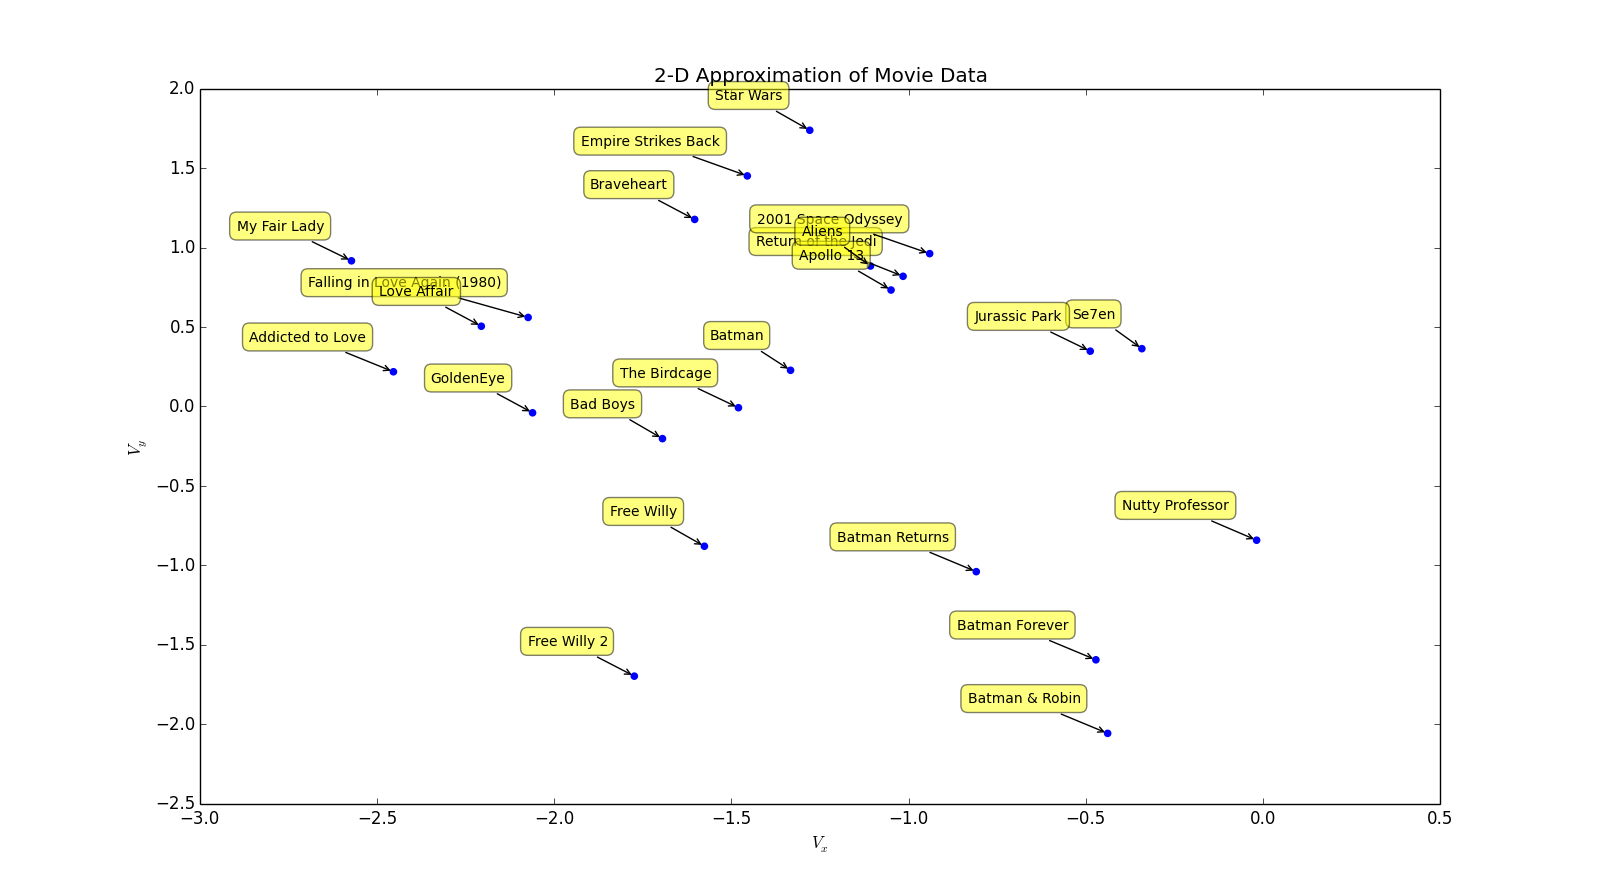
\includegraphics[width=1\textwidth]{final_graph_1}
There are some interesting trends in the above figure. Of course, since
this only captures 2 dimensions of a dataset which was significantly
higher-dimensional, we cannot capture all the variation in the movies.
We can observe, however, that there are clusters of similar movies
in this figure. Three of the Batman films seem to cluster towards the bottom
of the figure, with $V_{x}$ values varying between -1.0 and -0.25 and
$V_y$ values varying between -2.5 and -1.0. Furthermore, there is a group
of science-oriented or science fiction movies towards the top of the visual,
including movies like Aliens, Apollo 13, Space Odyssey. This cluster makes
sense because these movies all seem to revolve around similar thematic elements
of science, space, and generally futuristic tendencies. Of course, the Star Wars
films are also close together, all having $V_{y}$ positive and $V_x$ greater than
-1.75. The fact that 'Free Willy' and 'Free Willy 2' are relatively close
to each other shows sensible correlation. To conclude, we see that most of
the romantic and love-themed movies cluster towards lower $V_x$ values,
including Love Affair, Falling in Love Again, and Adicted to Love.

If we had to make some predictions on the axes of these graphs and what they
represent, we would guess that moving left on the $x$ axis correlated
to perhaps more emotional movies, or movies that appeal to females. Moving
higher on the $y$ axis seems to correlate to more science-based films. Although
the action films are generally scaterred, action films seem to be heavier
towards larger values of $V_x$.\\

As required, we also graph all the movies and users in one plot. Although
it's hard to interpret the meaning of the user data (the red dots below),
we can generally tell from this plot that both datasets are mean-centered
close to 0 in the $y$ direction (but maybe the movie dataset is negative-centric
in the $x$ direction). \\
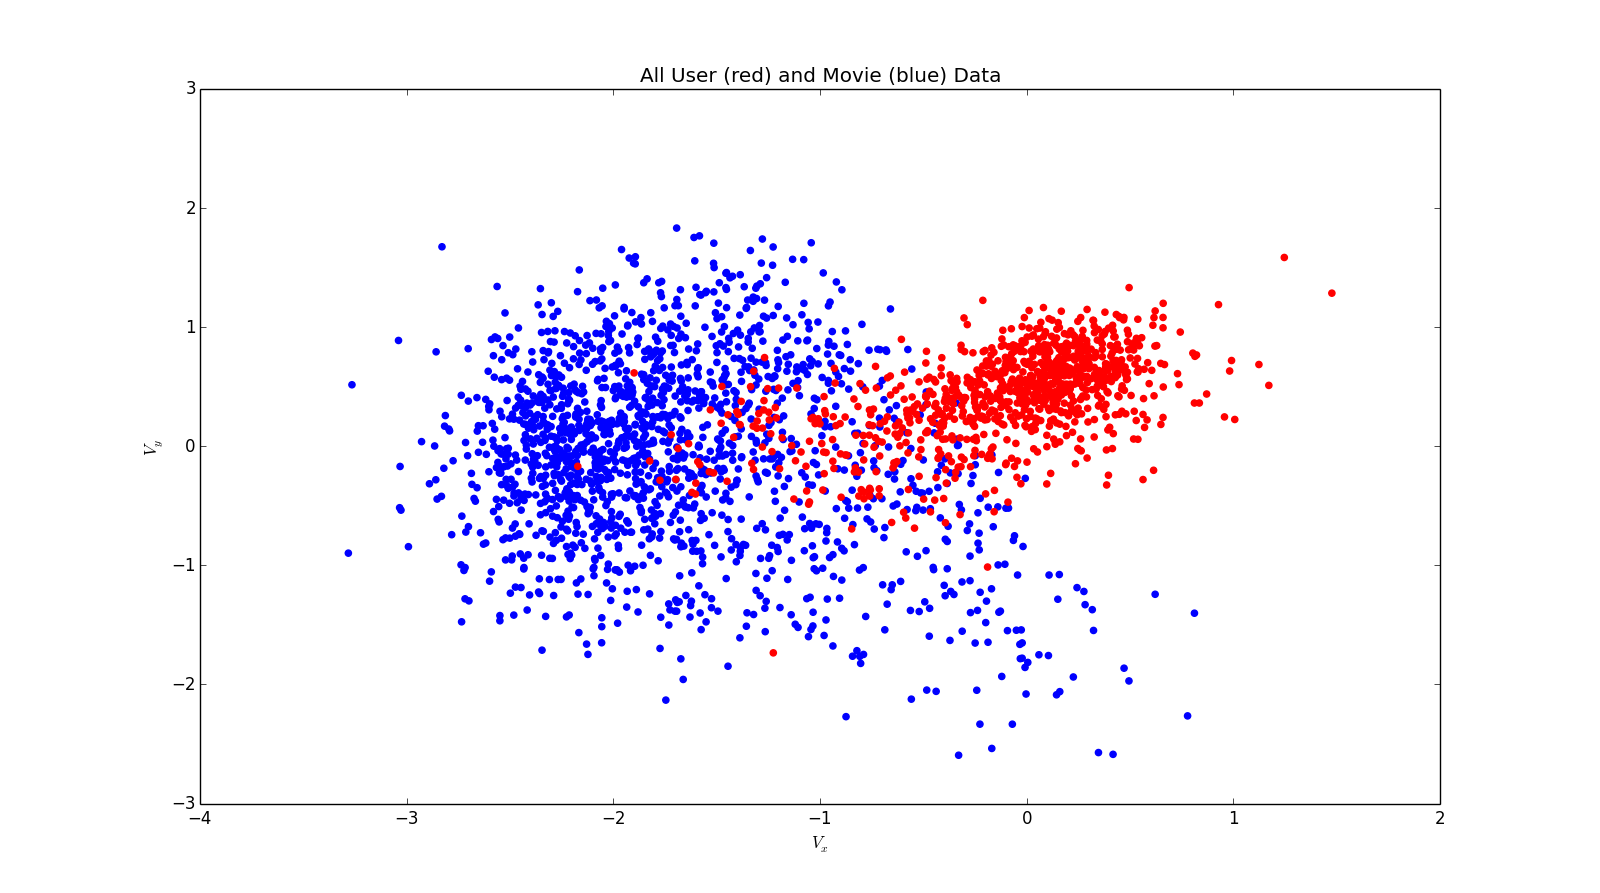
\includegraphics[width=1\textwidth]{all_users_movies}
To gain more insight, we picked out specifically the musicals from the set of movies
and highlighted them below in red. Since these movies are not all \textit{exclusively}
musicals, it's unreasonable to expect strong clustering. However, we see that
many of the musicals are indeed clustered between $-3 < V_x -1 $ and $0 < V_y < 1.5$.
We chose to graph musicals somewhat arbitrarily, but it seemed like the most
unique genre with the least overlap with other genres.
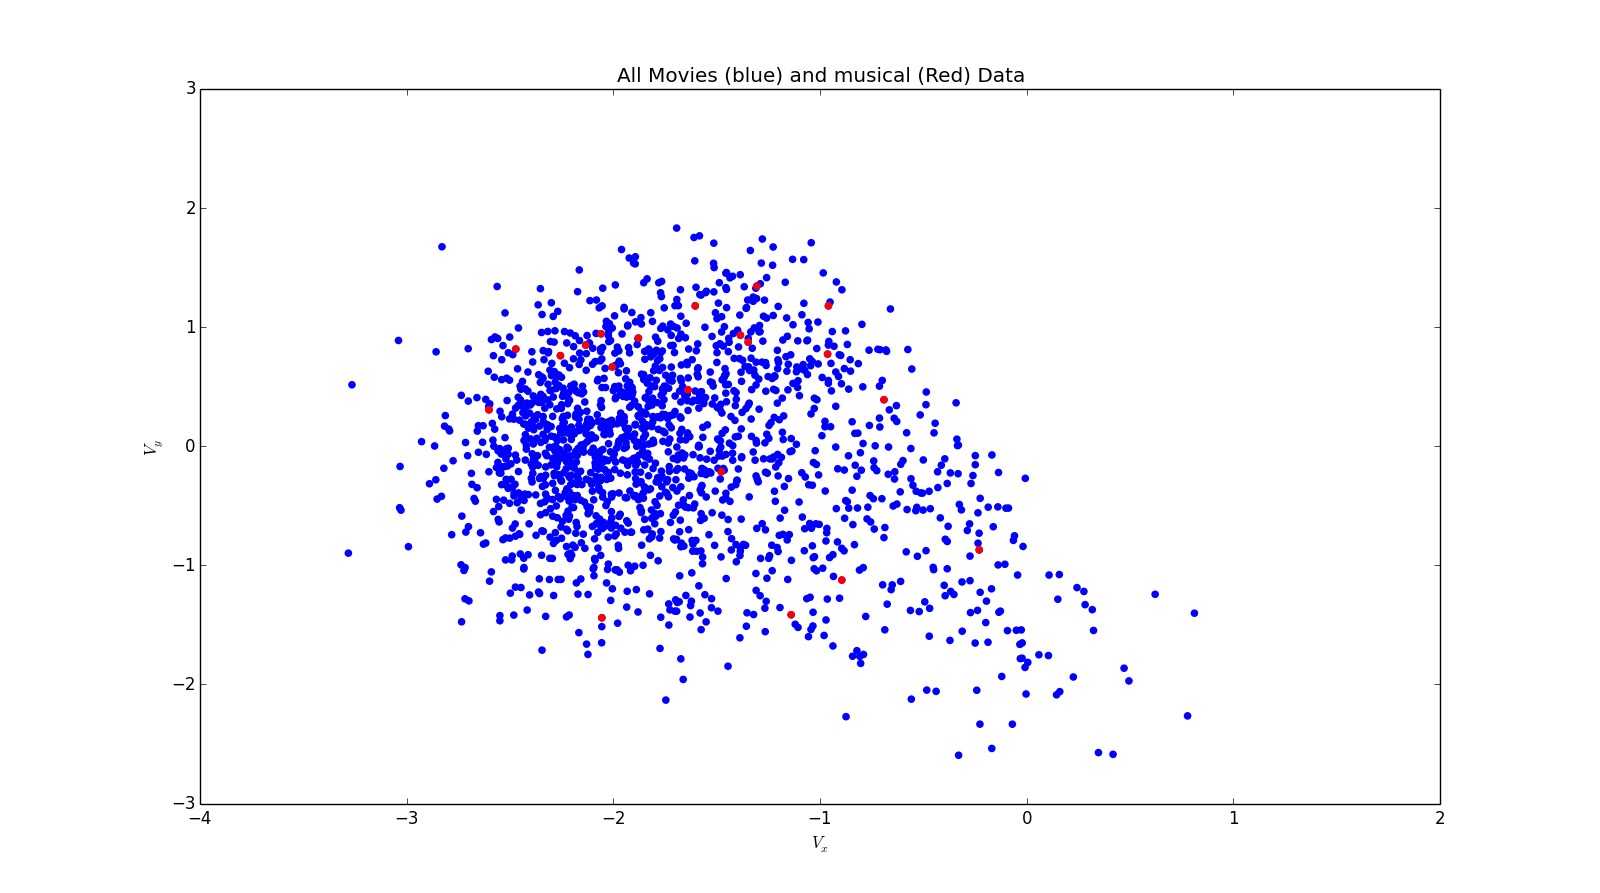
\includegraphics[width=1\textwidth]{musical_all_movies}

Furthermore, we calculated the average $v$ value for musicals: (-1.5548562, 0.3654483),
which makes aligns with our qualitiative observations.

\end{document}
